\subsection*{research}
i read the chapter in \autocite{experimental-rf} on oscillator design and
frequency synthesis, for a general survey of simple \vco design.

the first oscillator types discussed were simple \lc oscillators (hartley,
colpitts, clapp, seiler). the relevant figure from \autocite{experimental-rf}
is reproduced in figures \ref{fig:old-lc-oscillators} and
\ref{fig:less-old-lc-oscillators}.

\begin{figure}[H]
	\centering
	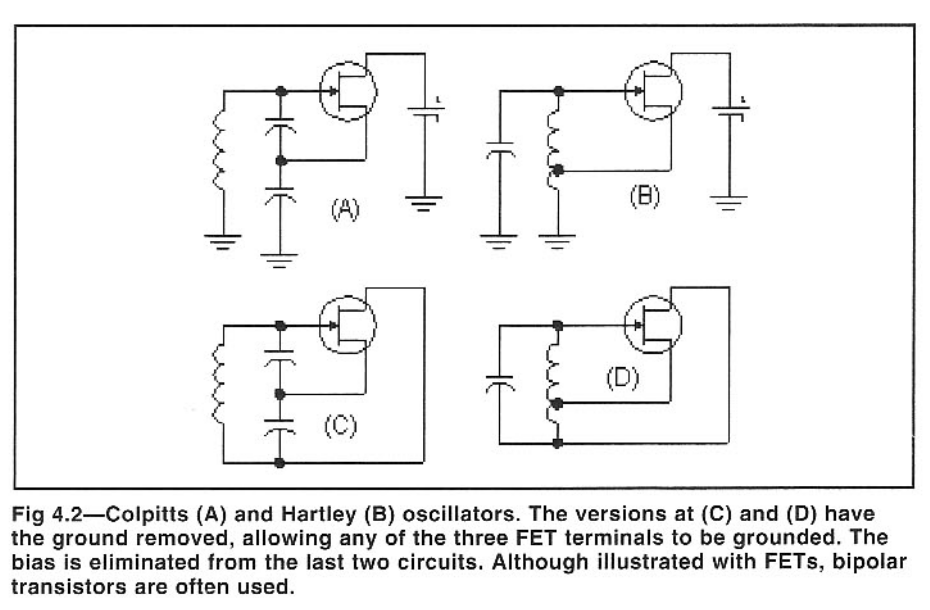
\includegraphics[width=.9\textwidth]{old-lc-oscillators.png}
	\caption{variants on the colpitts and hartley oscillators.}
	\label{fig:lc-oscillators}
\end{figure}

\begin{figure}[H]
	\centering
	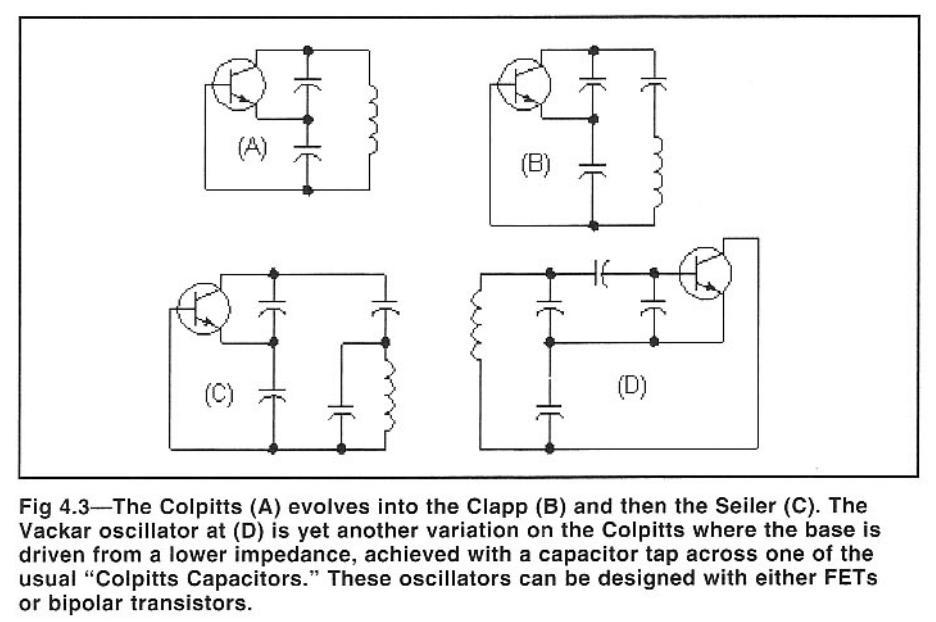
\includegraphics[width=.9\textwidth]{less-old-lc-oscillators.png}
	\caption{the clapp and seiler oscillators.}
	\label{fig:lc-oscillators}
\end{figure}
